
	\begin{titlepage}
		\begin{center}
			$$$$
			$$$$
			$$$$
			$$$$
			{\Large{НАЦИОНАЛЬНЫЙ ИССЛЕДОВАТЕЛЬСКИЙ УНИВЕРСИТЕТ}}\\
			\vspace{0.1cm}
			{\Large{ВЫСШАЯ ШКОЛА ЭКОНОМИКИ}}\\
			\vspace{0.25cm}
			{\large{Факультет физики}}\\
			\vspace{5.5cm}
			{\Huge\textbf{{Серия лабораторных работ по современной физике}}}\\%Общее название
			\vspace{1cm}
			{Работу выполнили студенты 3 курса}\\
			{Захаров Сергей Дмитриевич}\\
			{Еремин Валентин Антонович}\\
			{Святковская Ольга Алексеевна}\\
			\vfill
			
\includegraphics[width = 0.2\textwidth]{HSElogo}\\
			\vfill
			Москва\\
			2021
		\end{center}
	\end{titlepage}
	
\tableofcontents

\newpage

\section{Зависимость сопротивления материала от температуры}

\section{Зависимость вида ВАХ диода от температуры}

\section{Изучение эффекта Холла}
\subsection{Цели работы}

\begin{enumerate}
	\item Пронаблюдать эффект Холла 
	
	\item Определить знак носителей заряда в полупроводнике 
	
	\item Определить подвижность и концентрацию носителей
	
	
\end{enumerate}
\subsection{Теория эффекта}
\subsubsection{Тензор сопротивления в магнитном поле}
Уравнение движения заряженной частицы, на которую действует электрическое поле в плоскости распостранения заряда и магнитное поле перпендиклярно, можно записать как:
\begin{equation}
	 m\frac{d\textbf{v}}{dt}=q(\textbf{E}+\textbf{v}\times\textbf{B})-m\frac{\textbf{v}}{\tau} \\
\end{equation}
Где \textbf{v} - средняя по всем частицам скорость. 

Подвижностью носителей заряда будет называться коэффициент пропорциональности между дрейфовой скоростью носителей и приложенным электрическим полем при отсутствии магнитного: $\mu$=q$\tau$/m

Тогда в стационарном состоянии d\textbf{v}/dt = 0 в матричном виде:

\begin{equation}
\left(\begin{array}{ccc}
1 & -\mu B & 0 \\
\mu B & 1 & 0 \\
0 & 0 & 1
\end{array}\right)\left(\begin{array}{l}
v_{x} \\
v_{y} \\
v_{z}
\end{array}\right)=\mu\left(\begin{array}{l}
E_{x} \\
E_{y} \\
E_{z}
\end{array}\right)
\end{equation}
Вводя тензор спортивления: $\textbf{E}=\hat{\rho} \textbf{j} = ne \hat{\rho}\textbf{v}$, где n - концентрация носителей заряда получаем:
\begin{equation}
\hat{\rho}=\frac{1}{n e \mu}\left(\begin{array}{ccc}
1 & -\mu B & 0 \\
\mu B & 1 & 0 \\
0 & 0 & 1
\end{array}\right)
\end{equation}
И, соответственно, обратный тензор проводимости:
\begin{equation}
\hat{\sigma}=\frac{\hat{\sigma}_{0}}{1+(\sigma B)^{2}}\left(\begin{array}{ccc}
1 & \mu B & 0 \\
-\mu B & 1 & 0 \\
0 & 0 & 1
\end{array}\right),
\end{equation}
где $\sigma_0=ne\mu$.

\subsubsection{Подвижность и концентрация носителей. Схема снятия снятия напряжений}
Изучаемый образец (\ref{fig:sample2}) представляет из себя узкий и длинный прямоугольный параллелепипед с известными геометрическими параметрами. Токовые контакты (1 и 4) находятся на торцах образца, и ток, соотвественно течет вдоль продольного направления, а магнитное поле направлено ему перпендикулярно.

\begin{figure}[H]
	\centering
	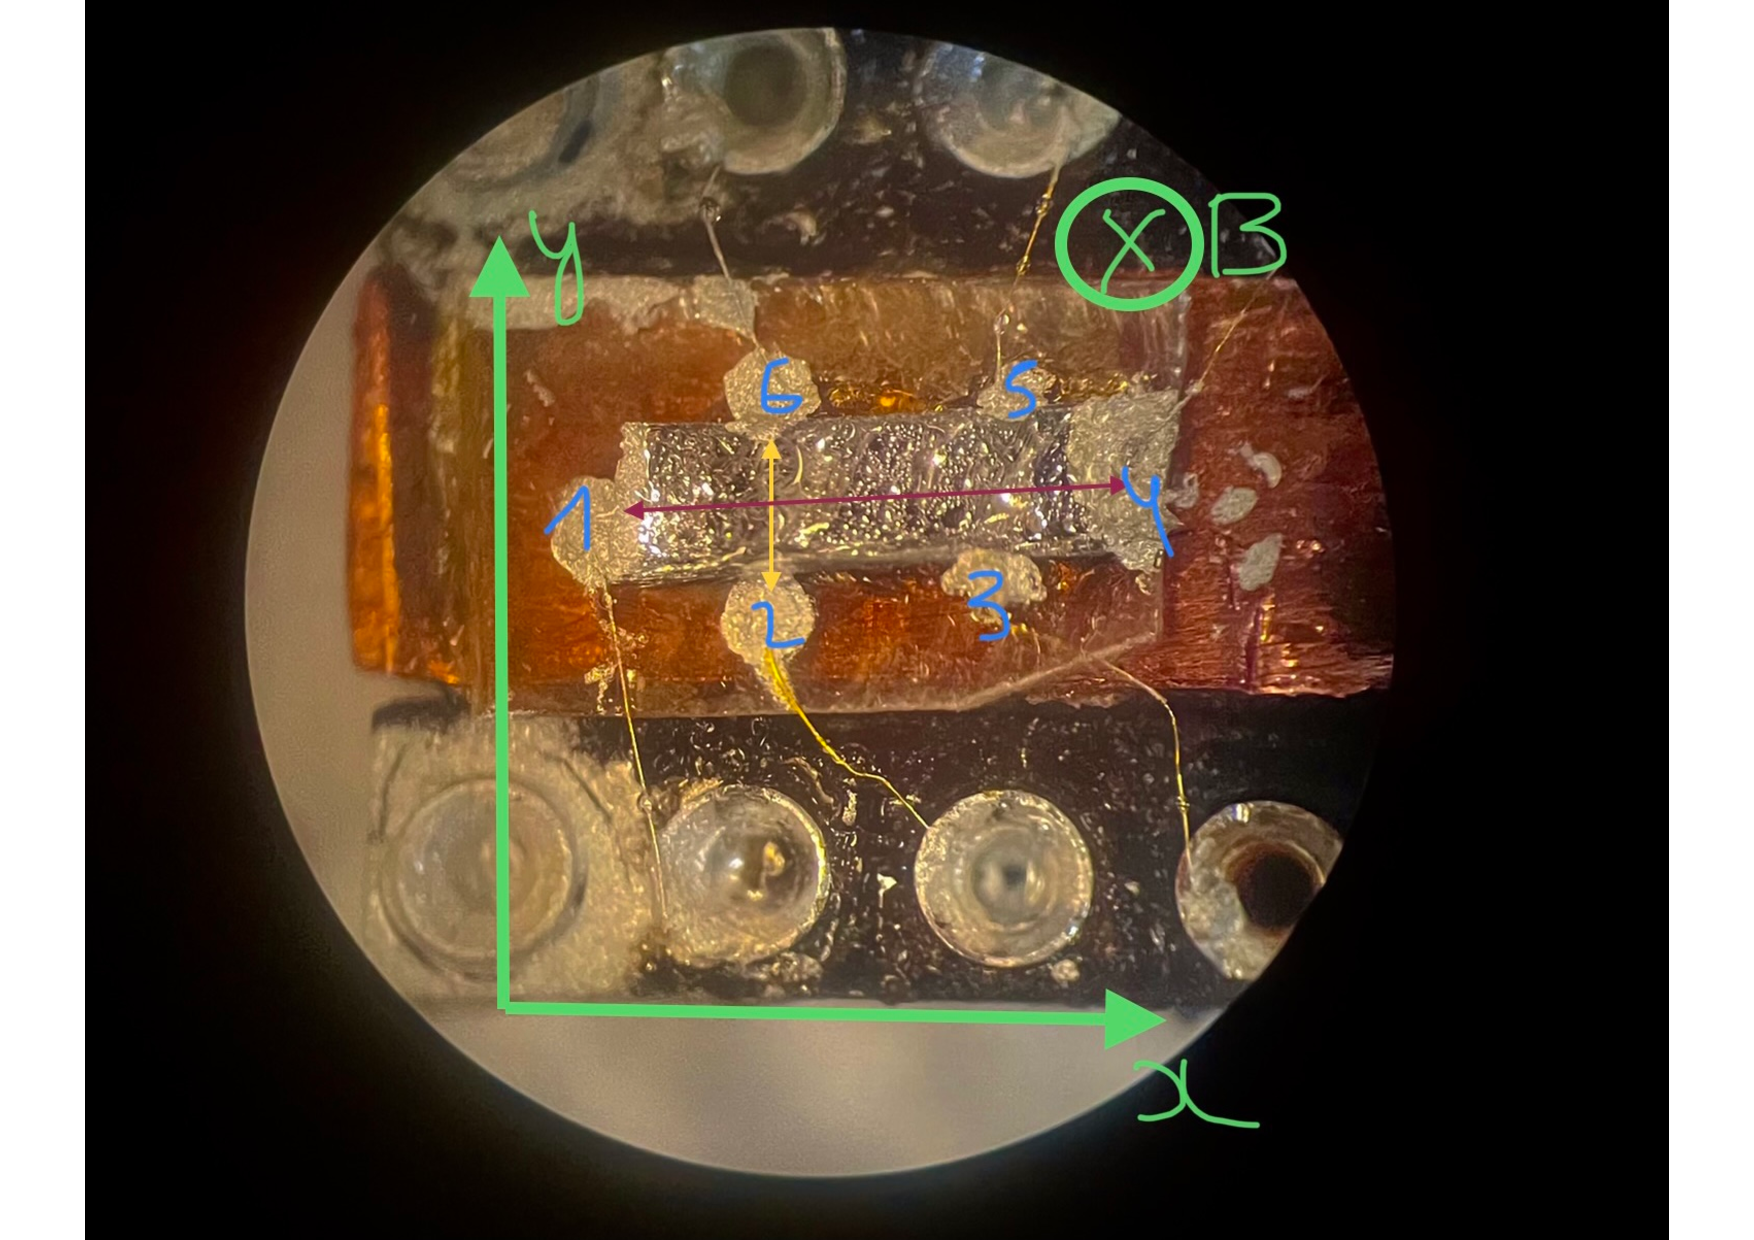
\includegraphics[width=\linewidth]{Sample2.pdf}
	\caption{Образец}
	\label{fig:sample2}
\end{figure}
Электроны под действием силы Лоренца будут отклоняться от направление тока и, соотвестсвенно, создавать разность потенциалов между краями образца (между 6 и 2, 5 и 3). То есть компонента электрического поля будет возрастать до тех пор, пока не компенсирует силу Лоренца. 

В установившемся состоянии тока вдоль оси y не будет, то есть: 
\begin{equation}
\left(\begin{array}{c}
j_x \\
0
\end{array}\right)=\frac{\hat{\sigma}_{0}}{1+(\mu B)^{2}}\left(\begin{array}{cc}
1 & \mu B \\
-\mu B & 1
\end{array}\right)\left(\begin{array}{c}
E_{x} \\
E_{y}
\end{array}\right)
\end{equation}
При этом $E_x=U_{xx}/l$ и $E_y=U_{xy}/w$, тогда
\begin{equation}
    \mu=\frac{1}{B}\frac{V_y}{V_x}\frac{l}{w}
\end{equation}
Также, зная направление тока и магнитного поля, а также знак холловского попречного напряжения, можно определить тип носителей заряда, соответсвующему знаку подвижности.

Записывая полный ток через образец, выразим его через концентрацию:
\begin{equation}
    I=j_xwh=(\sigma_{xx}E_x+\sigma_{xy}E_y)wh=\sigma_0 wh=ne\mu wh
\end{equation}
А следовательно
\begin{equation}
    n=(eh\frac{V_y}{IB})^{-1}
\end{equation}
\subsection{Ход работы}
\subsubsection{Калибровка магнита}
Калибровка магнита с помощью тесламетра позволила произвести взаимооднозначное соотвествие силы подаваемого тока и напряженности поля внутри магнита. Также было установлено соотвествие полярности подключения источника тока и направления поля. Результаты измерений приведены на графике (\ref{fig:calib}) Полученная зависимость: 26.2 mTl/1A

\begin{figure}[H]
	\centering
	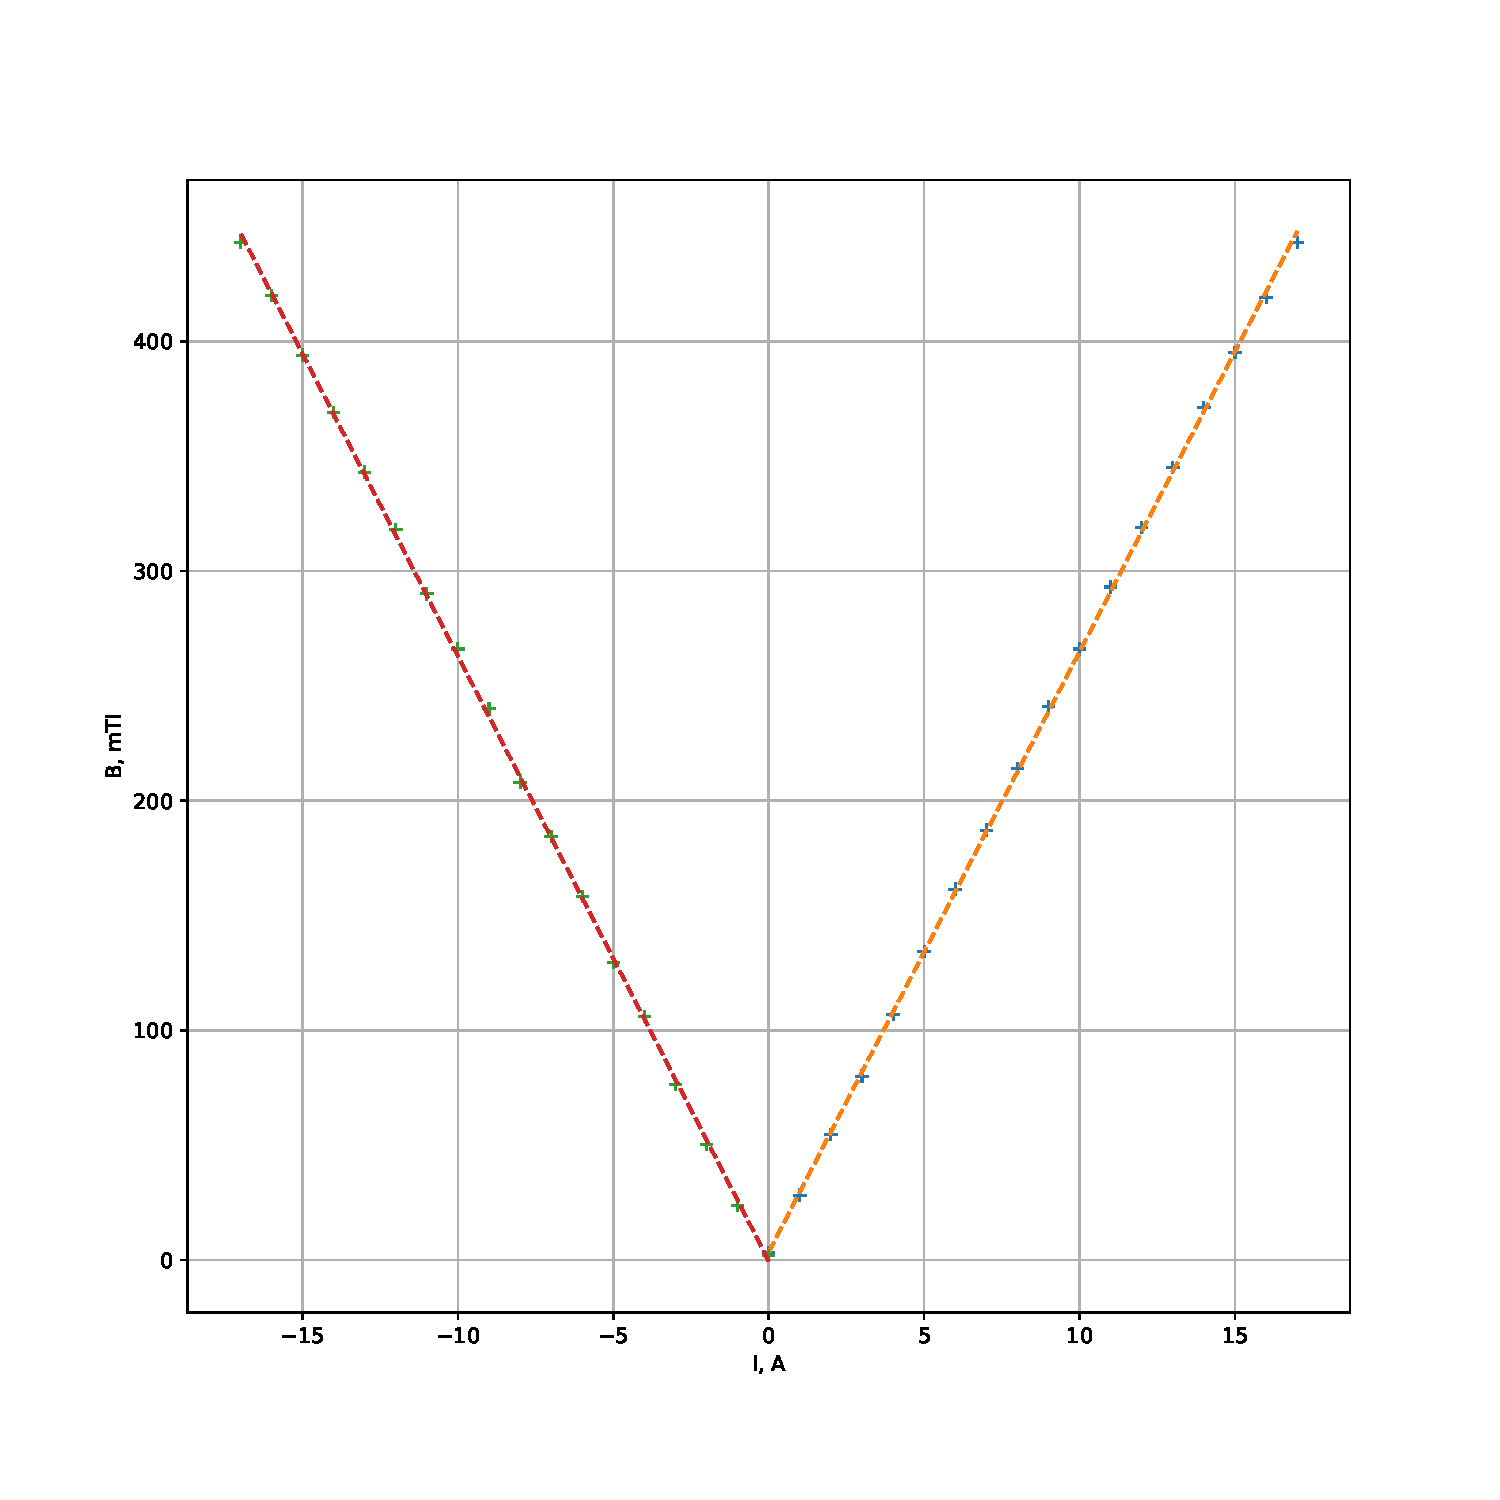
\includegraphics[width=0.7\linewidth]{Calibration.pdf}
	\caption{Зависимость напряженности поля от тока}
	\label{fig:calib}
\end{figure}

\subsubsection{Снятие данных зависимости продольного и поперечного напряжений от величины и направления магнитного поля }
Схема электрической цепи была собрана на вставке в криостат и разводящей коробке с общей землей, соединенной посредством внешним оплеток bnc-разъемов. Это позволяло легко переключаться между контактами для измерения продольного и поперечного  наряжений.

На встроенном в усилитель Lock-in генераторе было установлено напряжение 5V, в цепь последовательно был подкючен  5.05к-омный резистор. Такое спротивление много больше сопротивления на образце ($\sim$ 60 ом), а следовательно ток через полупроводник: $$I=5V/5.05kOhm\approx1mA$$

Далее образец помещался в магнитное поле и снималась зависимость продольного и поперечного напряжений от велечины индукции магнитного поля. Аналогичный опыт проводился после погружения образца в азот и, соответсвенно его охлажение до 77K.

\subsection{Обработка данных}
\subsubsection{Определение типа носителей заряда}
Как уже было сказано выше, тип носителей заряда определяется знаком подвижномсти и, соответсвенно, направлением Холловского электрического поля. 

На практике это происходило так: в конфигурации, изображенной на рисунке (\ref{fig:sample2}) ток был направлен вдоль оси x, а магнитное поле 'от нас'. Считывание напряжения выдавало разность потенциалов между контактами 2 и 6. Тогда в предположении, что носителями заряда являются электроны, на нижнем краю образца будет под действием силы Лоренца скапливаться отрицательный заряд, а на верхнем положительный. И соотвественно мы будет считывать отрицательное напряжение. В действительности же, в данной конфигурации мы наблюдали положительную разность потенциалов между контактами, что напрямую сведительствует о том, что носители заряда - дырки.
\subsubsection{Продольное напряжение}

Зависимость продольного сопротивления для T=77K (между контактами 6 и 5) представлено на рисунке (\ref{fig:long})

Теоретически, зависимости продольного сопротивления, а следовательно и напряжения, от велечины магнитного поля наблюдаться не должно. И действительно, разброс снятых величин составляет порядка 1 процента. Эти флуткуации можно обяснить неидеальным расположением контактов относительно направления тока (то есть возникновение холловского напряжения), слабой точность позиционирования образца в магнитном поле и т.д. 

Значения измеренного продольного напряжения для комнатной температуры:
$$V_{xx} = 229 \mu V  $$

Для 77K:
$$V_{xx} = 17.46 \mu V $$

\begin{figure}[H]
	\centering
	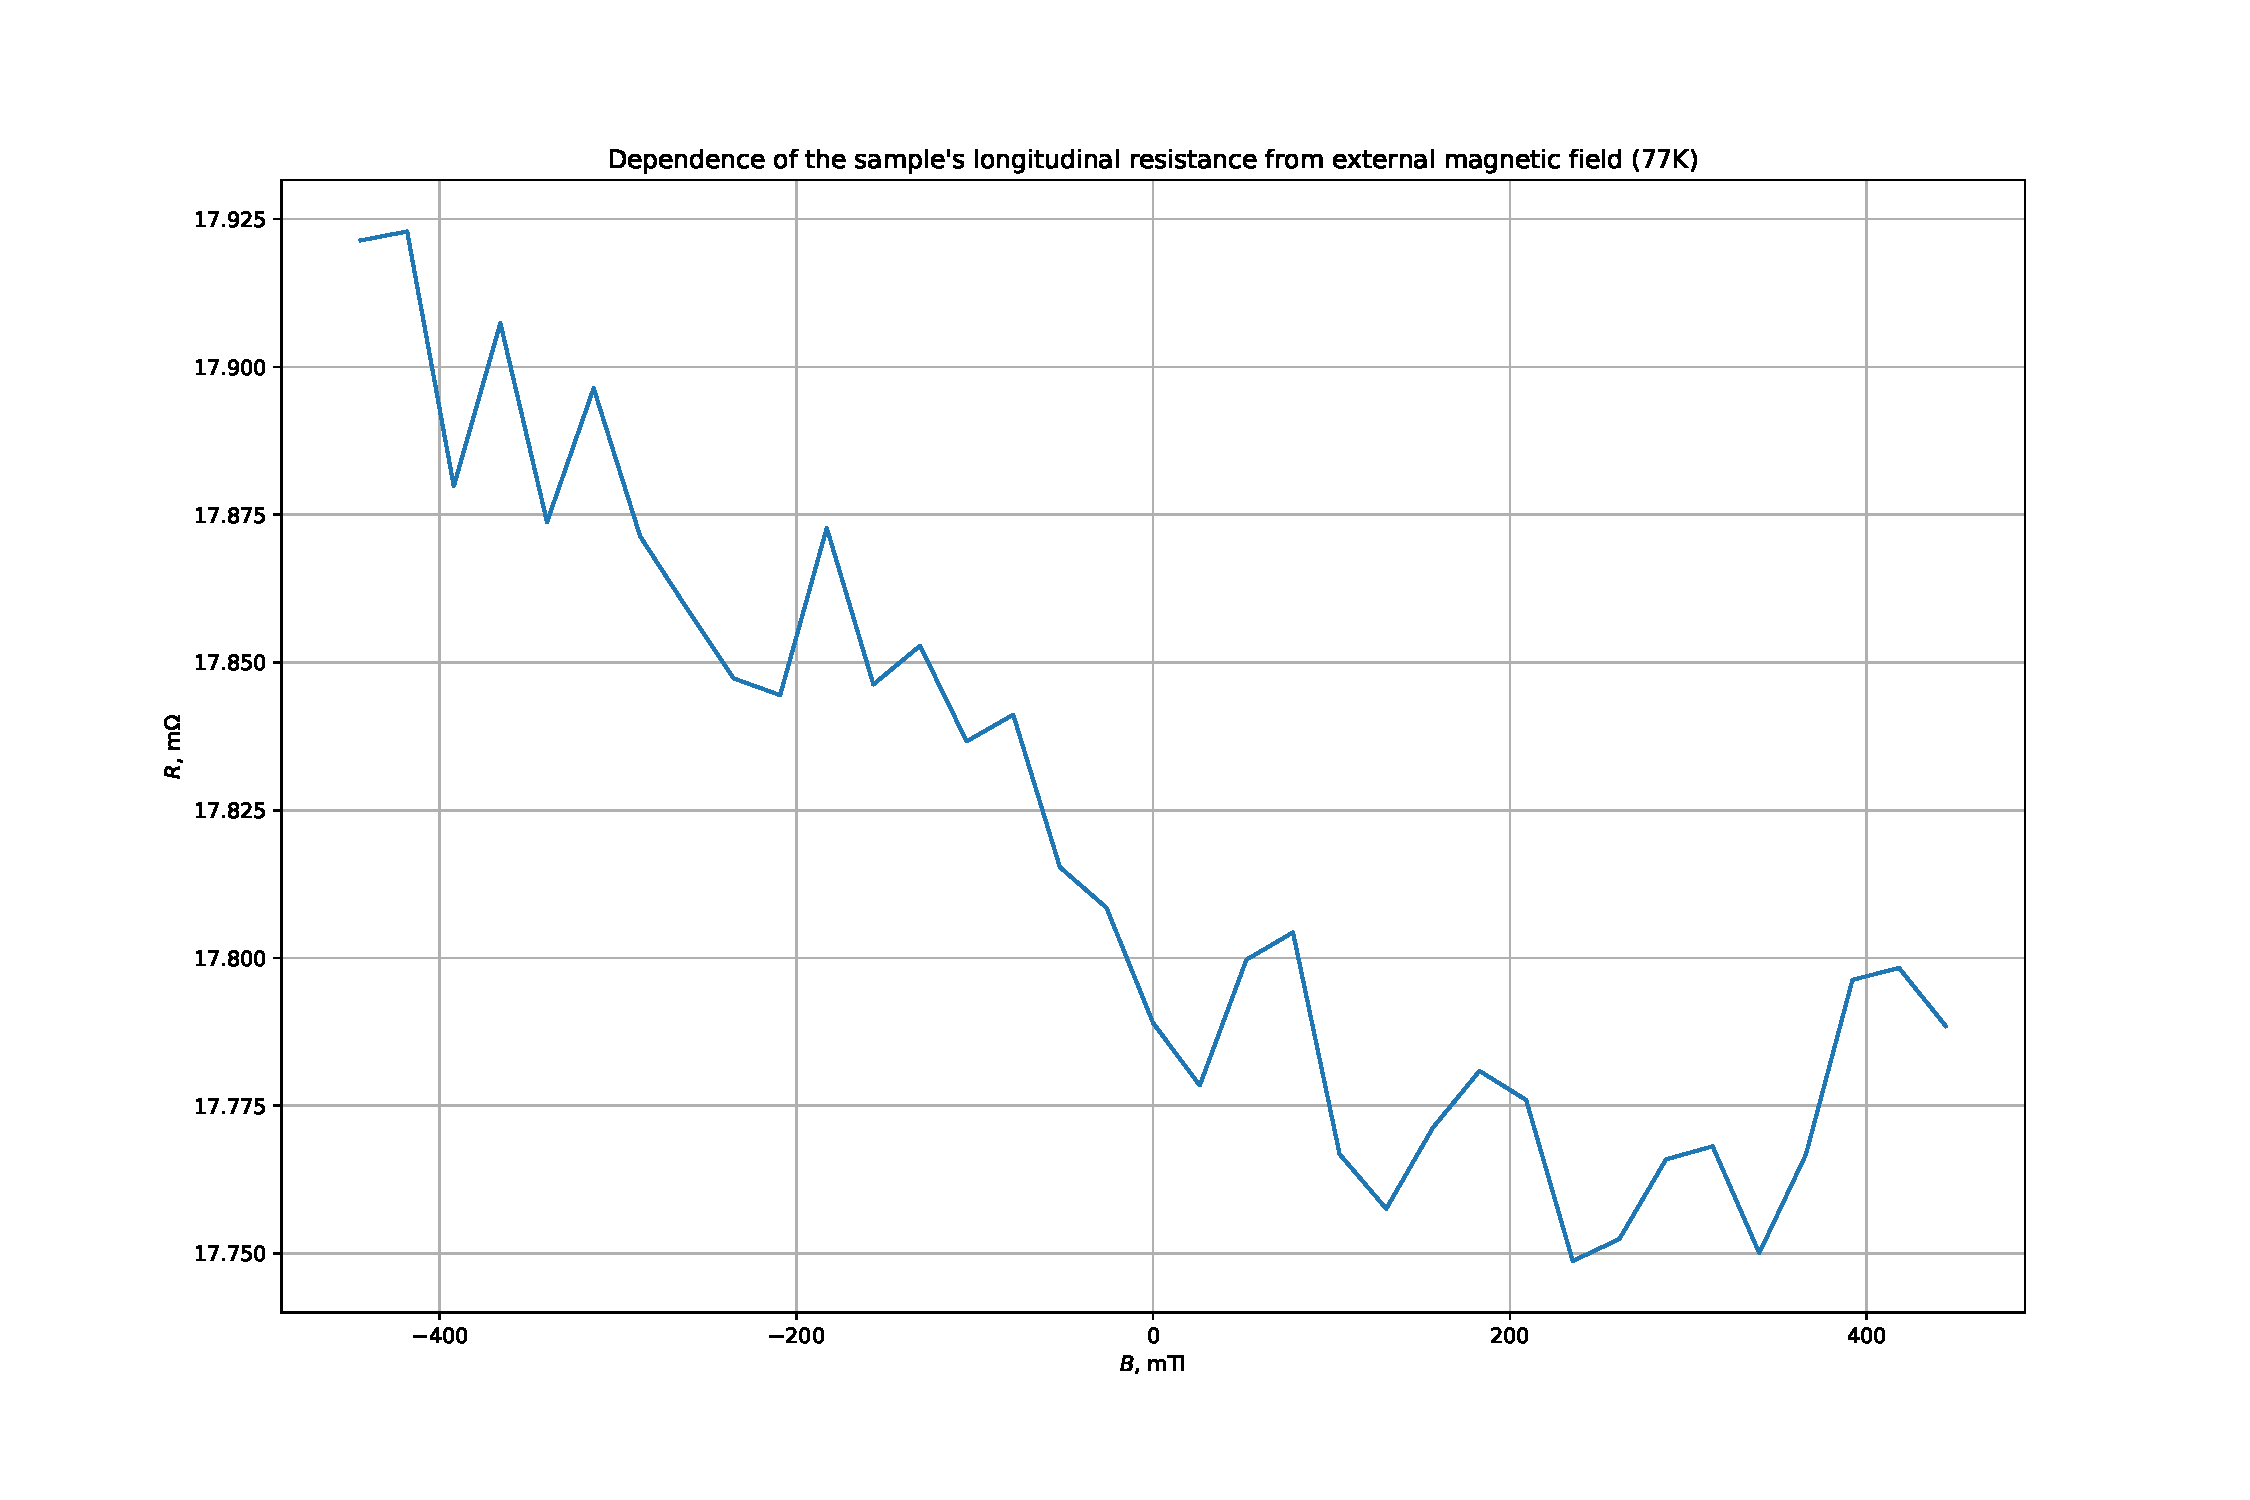
\includegraphics[width=\linewidth]{longitudunal.pdf}
	\caption{Зависимость продольного сопротивления от поля}
	\label{fig:long}
\end{figure}

\subsubsection{Поперечное сопротивление}

Данные зависимости Холловского сопротивления от величины индукции магнитного поля приведены на рисунке (\ref{fig:room}) для комнатной температуры и на рисунке (\ref{fig:cold}) для температуры азота.

Напомним формулы для подвижности носителей заряда и их концентрации:
$$\mu=\frac{1}{B}\frac{V_y}{V_x}\frac{l}{w};   n=(eh\frac{V_y}{IB})^{-1}  $$
При этом $V_y/IB = R_y/B$ - наклон прямой зависимости холловского сопротивления от магнитного поля. h - толщина образца - 180 мкм

Таким образом концентрация носителей заряда при температуре 77K:

$$n\approx15*10^{19}cm^{-3}$$ 

При комнатной температуре:
$$n\approx21*10^{19}cm^{-3}$$ 
\begin{figure}[H]
	\centering
	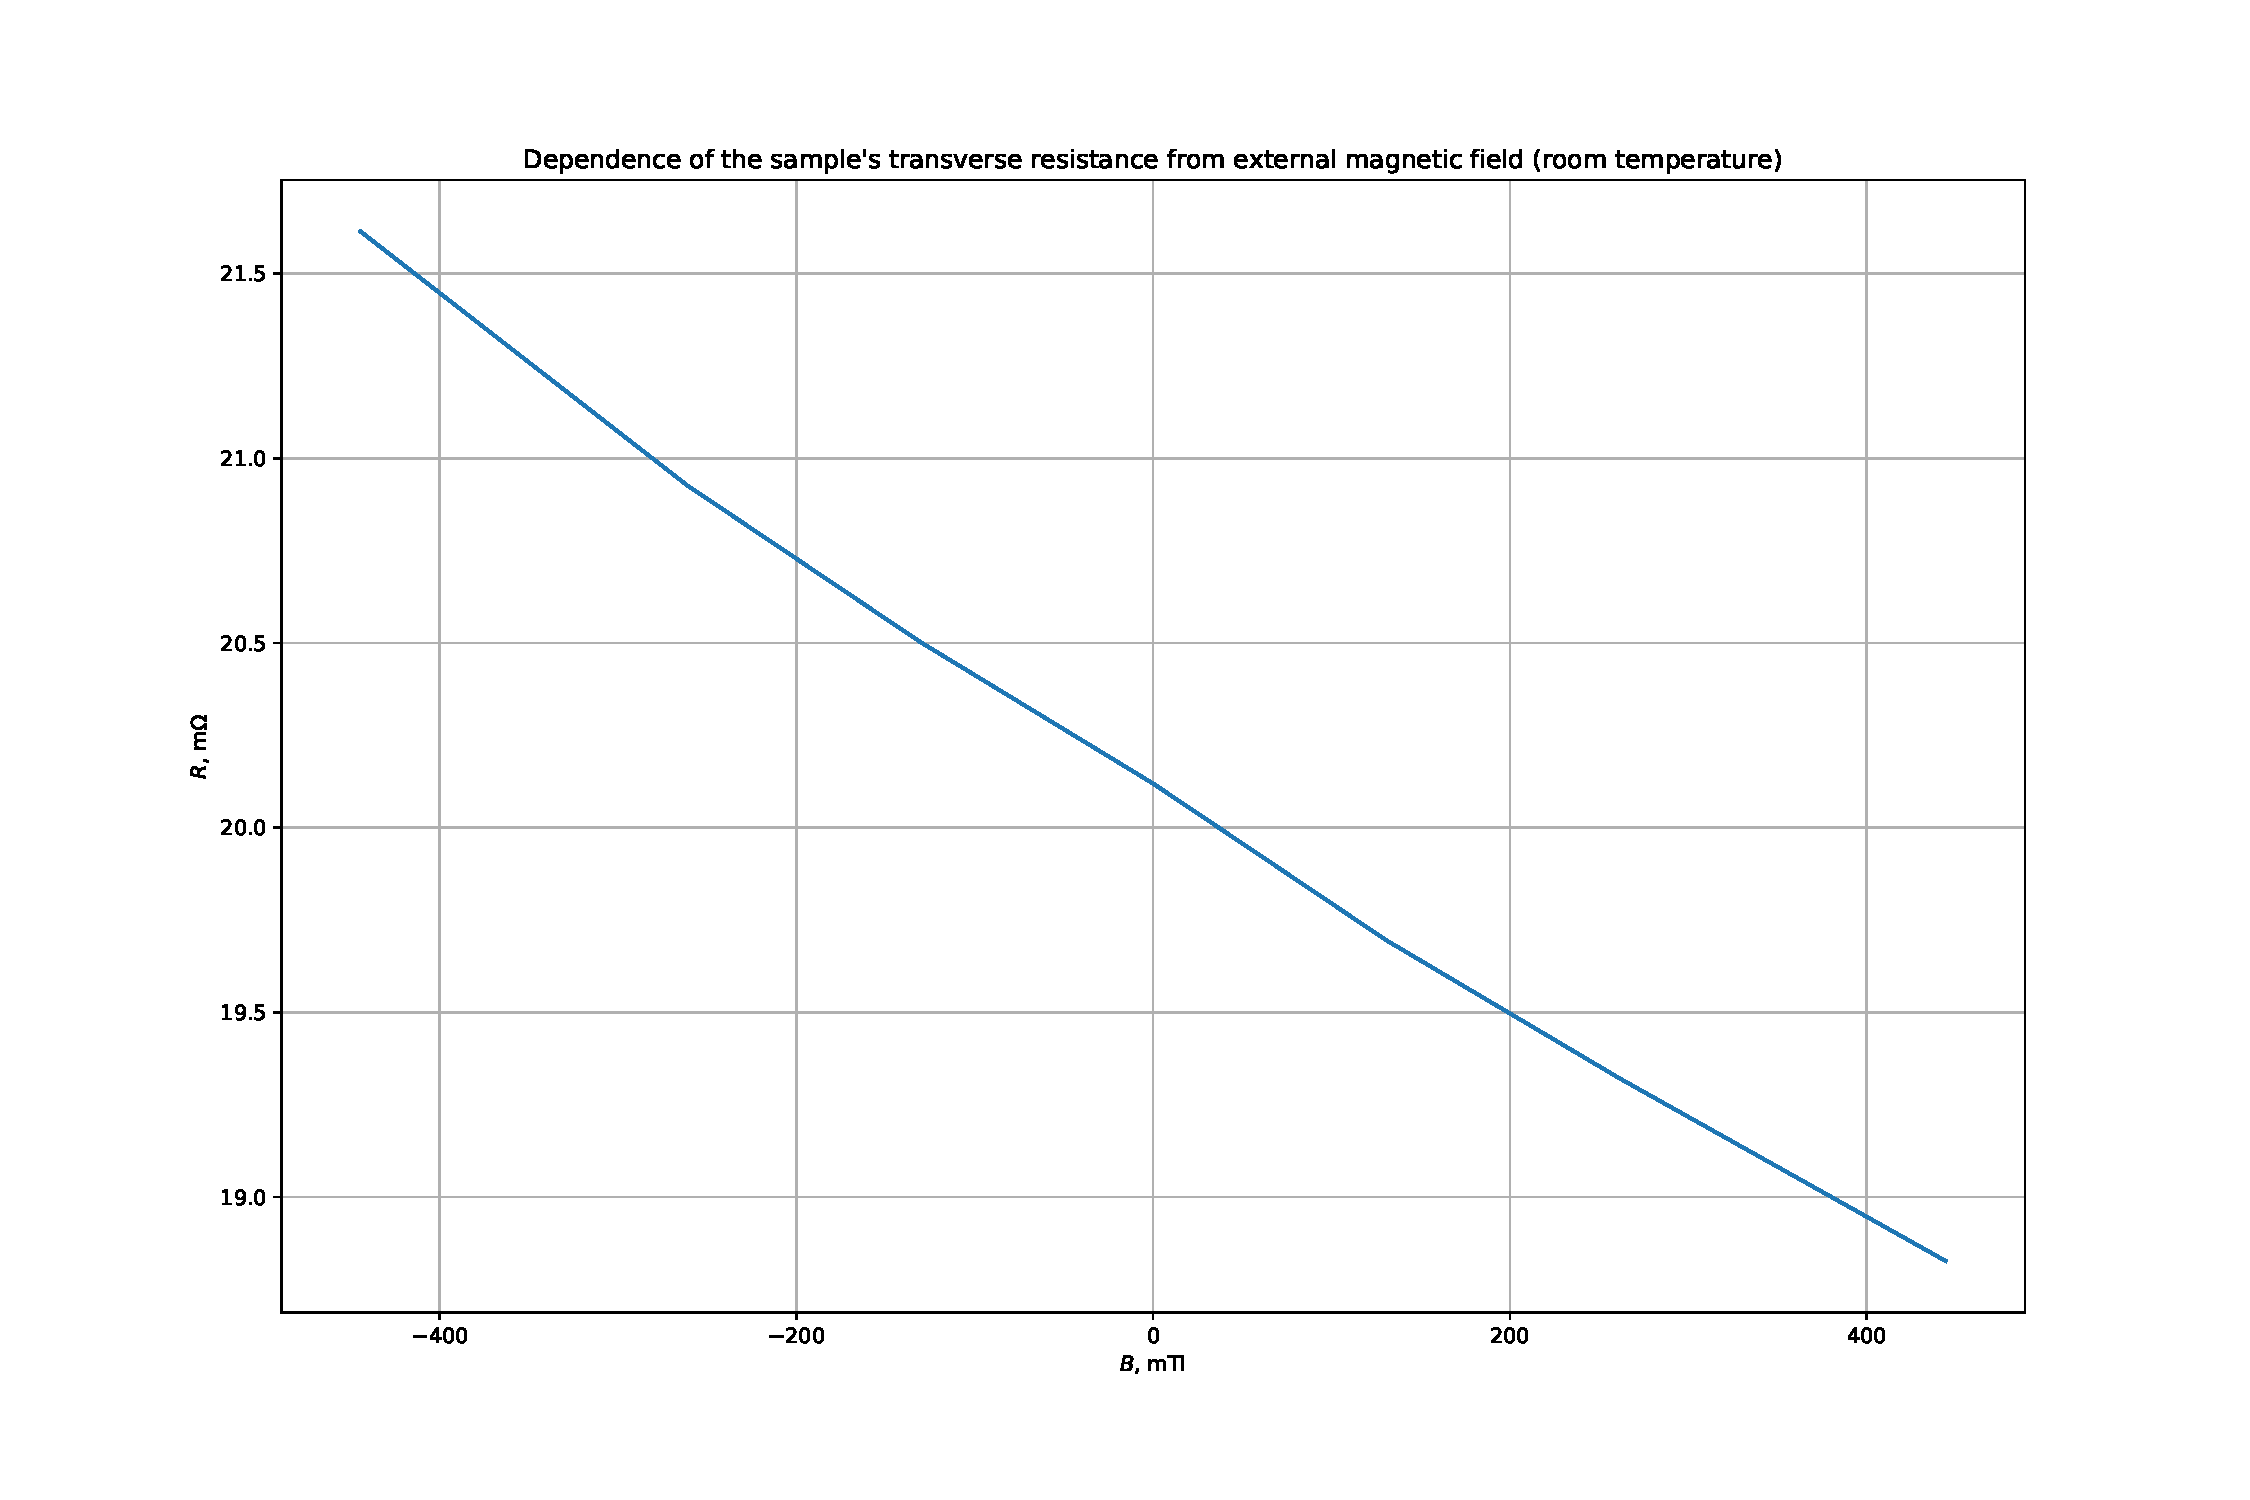
\includegraphics[width=0.8\linewidth]{room.pdf}
	\caption{Зависимость поперечного сопротивления от поля(комнатная температура)}
	\label{fig:room}
\end{figure}

\begin{figure}[H]
	\centering
	\includegraphics[width=0.8\linewidth]{cold.pdf}
	\caption{Зависимость поперечного  сопротивления от поля (азот)}
	\label{fig:cold}
\end{figure}

Измеряя отношение расстояний между продольными и попречными контактами: $l_1$/$w$=1.7, находим значение подвижности при комнатной температуре:
$$\mu\approx 0.72   m^2/V*s$$

И при 77K:

$$\mu\approx 3.2   m^2/V*s$$

Наблюдаемый эффект возникновения поперечного напряжения линеен по полю. При этом заметим, что при нулевой напряженности магнитного поля, вопреки теоретическому ожиданию, все равно существует ненулевое напряжение. Объясняется это, как уже было сказано выше, неточностью расположения контактов и рядом других факторов. 

Тогда симметризацией тензора напряжения и сопротивления мы получим постоянное значение, а антисимметризацией линейное по полю:

$$ \rho_{xx}=\frac{R(B)+R(-B)}{2};\rho_{xy}=\frac{R(B)-R(-B)}{2}$$

Подставляя измеренные значения получаем для 298K:

$$\rho_{xx}\approx20,1 \text{mOhm};\rho_{xy}\approx0.00312*B \text{m$\omega$}$$

И для 77K:
$$\rho_{xx}\approx7,9 \text{mOhm};\rho_{xy}\approx0.00238*B \text{m$\omega$}$$
